\documentclass[10.9pt]{article}

\usepackage[paper=letterpaper,centering,margin=1.0in]{geometry}
\usepackage{setspace}

\usepackage[american]{babel}
\usepackage{epsfig,subfigure}
\usepackage{color,cite}
\usepackage{amsthm,amsfonts,amsmath,amssymb,amstext,latexsym}
\usepackage{multirow}
\usepackage{soul}
%\usepackage{xxcolor}
\usepackage{xcolor}
%\usepackage{hyperref}
\usepackage{algorithm}
\usepackage{algpseudocode}

\usepackage{graphicx}
\usepackage{amstext}

%\usepackage[utf8]{inputenc}
%\usepackage{enumitem}

%\algnewcommand{\IIf}[1]{\State\algorithmicif\ #1\ \algorithmicthen}
%\algnewcommand{\EndIIf}{\unskip\ \algorithmicend\ \algorithmicif}
\newcommand{\algorithmicbreak}{\textbf{break}}

\newcommand*{\Cdot}[1][1.25]{%
  \mathpalette{\CdotAux{#1}}\cdot%
}
\newdimen\CdotAxis
\newcommand*{\CdotAux}[3]{%
  {%
    \settoheight\CdotAxis{$#2\vcenter{}$}%
    \sbox0{%
      \raisebox\CdotAxis{%
        \scalebox{#1}{%
          \raisebox{-\CdotAxis}{%
            $\mathsurround=0pt #2#3$%
          }%
        }%
      }%
    }%
    % Remove depth that arises from scaling.
    \dp0=0pt %
    % Decrease scaled height.
    \sbox2{$#2\bullet$}%
    \ifdim\ht2<\ht0 %
      \ht0=\ht2 %
    \fi
    % Use the same width as the original \cdot.
    \sbox2{$\mathsurround=0pt #2#3$}%
    \hbox to \wd2{\hss\usebox{0}\hss}%
  }%
}


%\algdef{SE}[SUBALG]{Indent}{EndIndent}{}{\algorithmicend\ }%
%\algtext*{Indent}
%\algtext*{EndIndent}



\newcommand{\squishlist}{
 \begin{list}{$\bullet$}
  { \setlength{\itemsep}{0pt}
     \setlength{\parsep}{3pt}
     \setlength{\topsep}{3pt}
     \setlength{\partopsep}{0pt}
     \setlength{\leftmargin}{1.5em}
     \setlength{\labelwidth}{1em}
     \setlength{\labelsep}{0.5em} } }

\newcommand{\squishend}{
  \end{list}  }

\newtheorem{theorem}{Theorem}
\newtheorem{lemma}{Lemma}
\newtheorem{conjecture}{Conjecture}
\newtheorem{remark}{Remark}
% \newtheorem{proof}{Proof}
\newtheorem{proposition}{Proposition}
\newtheorem{observation}{Observation}
\newtheorem{definition}{Definition}
\newtheorem{corollary}{Corollary}
\newtheorem{assumption}{Assumption}

\newcommand{\bydef}{\stackrel{\rm{def}}{=}}
%\newcommand{\textul}[1]{\underline{#1}}

\newcommand{\cP}{{\cal P}}
\newcommand{\cR}{{\cal R}}
\newcommand{\cK}{{\cal K}}
\newcommand{\norm}[1]{\left\Vert#1\right\Vert}
\newcommand{\mc}[1]{\mathcal{#1}}
\newcommand{\Lrz}{\mbox{${\mathbb L}$}}
\newcommand{\DMU}{\text{DMU}}


% Comments colors conventions
\newcommand{\J}[1]{{\textcolor{cyan}{#1}}}
\newcommand{\JC}[1]{\textbf{{\textcolor{red}{Juan: #1}}}} 
\newcommand{\SAB}[1]{\textbf{{\textcolor{orange}{Sab: #1}}}} 

\newcommand{\preg}[1]{\textbf{{\textcolor{blue}{Sab: #1}}}} 


\def\R{\mbox{${\mathbb R}$}}           % Real numbers
\def\N{\mbox{${\mathbb N}$}}           % Natural numbers
\def\Z{\mbox{${\mathbb Z}$}}           % Integer numbers

\def\E{\mbox{${\mathbb E}$}}           % Expected value


\title{ Whisper Project \\ 
\begin{large} - Initial Report - }

\author{
\begin{center}
    \begin{tabular}[c]{  p{3.3cm}  p{3.3cm}  p{3.3cm} }
		Fernando Villa & Khalid Alobaid & Mariya Abdiyeva \\
		Nicolas Cabuli & Oluremi Obolo & Santiago Arrubla
    \end{tabular}
\end{center}
}



%\author{Fernando Villa \and Khalid Alobaid \and Mariya Abdiyeva \and Nicolas Cabuli \and Oluremi Obolo \and Santiago Arrubla}

\begin{document}
\date{7 Febraury 2017}
\maketitle


\section{Project Description}
\label{sec:part 1}

\subsection{Requirements (Aims)}

Our aim is to create a distributed chat system with the following specific requirements by  priority.

\begin{table}[ht]
\caption{Requirements by priority level}
\label{tab:requirements}
    \begin{tabular}[c]{ | p{5cm} | p{5cm} | p{5cm} |}
		\hline
		\centering\textbf{Priority 1} & \centering{\textbf{Priority 2}} & \centering\textbf{Priority 3} &
    \hline
    \parbox[t]{5cm}{-Secure connection\\-Encrypted messages\\ -iOS, Android and Web platforms (at least two platforms)\\ -Contact list\\ -Search for contacts\\ -Sign in by email or Gmail \\ -One to one conversation (text message)} &  \parbox[t]{5cm}{-Send images\\ -Group chat\\ -Chat bubbles instead of username\\ -Notifications of received messages}
& \parbox[t]{5cm}{-Sign Up with Facebook\\ -Availability to send other type of media (e.g. video, voice notes, etc.)\\ -Online status of other users\\ -Acknowledgment of received, delivered and read messages, including date time\\ -Ability to use the chat offline}\\
    \hline
    \end{tabular}
\end{table}


\subsection{Strategy and Timetable}

Our strategy is to develop three client-based platforms (i.e. Android, iOS and Web) using Firebase as a server. The reason for including a third platform is to act as a backup should there be problem with any of the platforms during testing which we are unable to debug at the end. The tentative timetable (Figure ~\ref{fig:timetable}) presents the main activities required to complete our final product. It is important to state that the timetable and our strategy is constructed based on the Scrum ~\cite{scrum} methodology, which  is an agile software development guide that allows us to iterate and make incremental and evolutionary contributions.  We will also use different Project Management roles like a Scrum Master (who removes team obstacles and pushes resolutions) and the product owner (who acts as the client voice) to ensure a high-quality product. The main activities are explained as follows: 

\begin{enumerate}
	\item \textbf{Plan}: Here we defined how we are going to work, our goals and organization as a team. We also discussed our individual strengths and weaknesses and the tools available to achieve our aim and objectives.
	\item \textbf{Firebase}: For simplicity, costs (free) and security we are using this Backend as a Service platform to have a robust system which takes care of the authentication, rules for accessing the database (read/write) and the storage of documents so that we could focus on the core functionality, i.e. the actual messaging.
	\item \textbf{UI}: Refers to designing the User Interfaces for all the clients.
	\item \textbf{Client Development}: This is the development of the specific application for each type of client (Android, iOS and Web): 
	\begin{enumerate}
		\item \textbf{Setup}: Here we add the required files and initialize the repository on GitHub. Then we create the project on Firebase so that we could share the same API Keys.
		\item \textbf{Login}: Build the login page, authentication using email and password, Gmail and Facebook if possible.
		\item \textbf{Conversations}: Text messaging between clients using Firebase as a central database containing the messages between recipients and taking care of the encryption. Add chat bubbles, send and receive messages, show them in an organized manner with timestamps.  
		\item \textbf{Image Message}: Share images inside messages (nice to have).
	\end{enumerate}
		\item \textbf{Integration Testing}: Test functionality across platforms. 
		\item \textbf{Quality Assurance}: Check that all clients communicate with the backend as intended in order to ensure that we cover all the required functionalities and fix any problem that we may have.	
\end{enumerate}

\begin{figure}[ht]
%[Parzen Window Estimated Distributions]
\centering
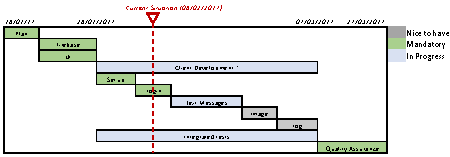
\includegraphics[width=0.9\textwidth]{figs/Timetable}
	\caption{Timetable}
	\label{fig:timetable}
\end{figure}


Please note that our activities in the client development are organized by hierarchy over time. Thus, developing the text message functionality (which is mandatory) is more important than the image message functionality (which is optional but highly desirable). Consequently, we decomposed our activities into tasks and allocated them to each team member as follows:

\begin{figure}[ht]
%[Parzen Window Estimated Distributions]
\centering
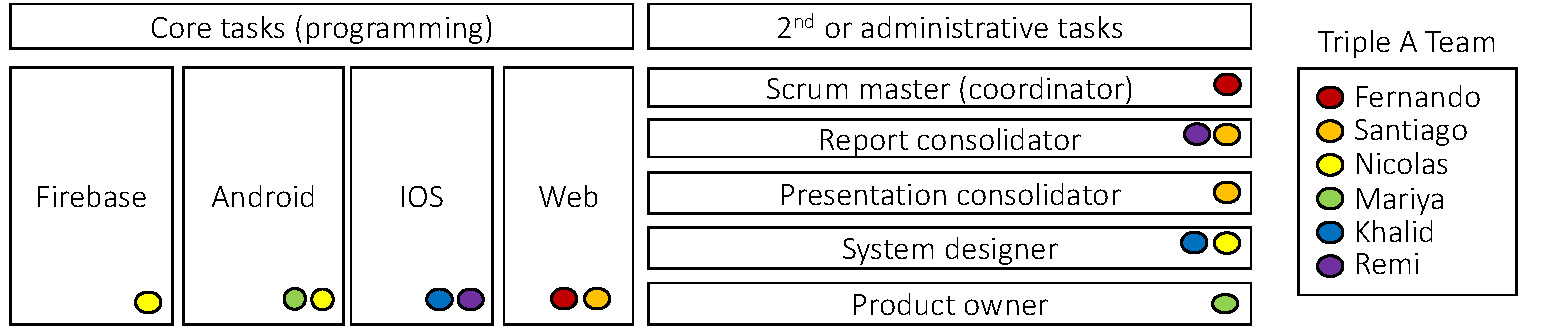
\includegraphics[width=1\textwidth]{figs/tasks}
	\caption{Tasks allocation}
	\label{fig:Tasks}
\end{figure}

\subsection{Current State}
Currently, we have developed the authentication functionality inside the three clients. Firebase authorizes the logged users and allows them see the data only if they are logged in.

\subsection{Next Steps}
Following our timetable, we are going to focus on making the proper database structure (chats, messages, users, receiver, sender, type of message, etc), rules for accessing the data inside the database (only user x and user y can see their own conversation) and adding new data to the database.

\section{Project Organization}
\label{sec:part 2}
In this section, we give more details about our organization, including how we will make decision and resolve conflicts. 

\subsection{Roles}

Every team member has two types of tasks: core tasks (e.g. programming goals) and administrative tasks (e.g. documentation and updating GitHub). Additionally, the coordinator is the official team communicator. However, it is clarified that this role does not imply a position of leadership or decision making (the decisions are jointly made by following the decision making and conflict resolution methodology in Section 2.4). The specific roles were already stated in Figure ~\ref{fig:Tasks}. However, those roles aren't definite and may change according to the project needs.

\subsection{Tools for Communication and Collaboration}

\begin{itemize}
	\item Slack (for communication purposes and specific tasks).
	\item GitHub (for code sharing and version control).
	\item Compulsory weekly "stand-up" every Monday (12:00 PM - 2:00 PM).
	\item Compulsory Google Hangout every Sunday (5:00 PM- 6:00 PM).
	\item Extra Google hangout meeting (when needed).
	\item Meeting on Wednesdays 2:00 PM- 5:00 PM (if needed). 
	\item A timetable and advance curve control (i.e. where we are vs where we ought to be).
	\item Our decision-making and conflict resolution methodology (Section 2.4).
	\item Learning meeting (each 15th day we discuss what we can improve as a team).
\end{itemize}




\subsection{Peer Assessment Criteria}

Our assessment methodology is based on the following set of criteria.

\begin{table}[ht]
		\caption{Assessment Criteria}
		\label{tab:requirements}
    \begin{tabular}[r]{ | p{2.2cm} | p{13.3cm}|}
		\hline
		\centering\textbf{Criteria} & \centering\textbf{Description} &
		\hline
		Amount of work & Amount of work that each member contributes (e.g. difficulty or complexity in the sub-set of requirements achieved by the member). \\
    \hline
		Team work skills & i) communication skills, ii) cooperation (e.g. how a member supports others) and willingness to resolve conflicts or reach agreements.\\
    \hline
		Proactiveness & Self-motivation to explore and propose new alternatives or options to overcome any difficulty. These include initiative, willingness to learn, good attitude to explore new things, enthusiastic, creativity and innovation.\\
    \hline
    \end{tabular}
\end{table}

Each member evaluates others on a scale of 1 and 5 (where 1 is the lowest and 5 is the highest score). For each criterion, each member would write a little justification, which could be replied by the other member. After-wards, the evaluator could decide to modify his assessment or otherwise. The final score of each member will be the average of all the valuations, weighted by the weight of each criterion (i.e. $1/3$). Then, the $100$ points would be proportionally distributed to meet with the assessment criteria of the module. 


\subsection{Decision Making, Agreements and Conflict Resolution Methodology}

Making agile agreements and rapidly resolving conflicts are key factors towards maximizing our team output. Our methodology is inspired by the agents and multiagents theory ~\cite{BDI}, specifically in a practical reasoning agent BDI (Belief – Desires - Intentions).  In this manner, every team member possesses a valid point of view. Any difference between opinions goes through a deliberation process (where personal conflict is a conciliation process, which is a special type of deliberation), that would transform a set of options or desires to a set of intentions (this implies that each time there is a deliberation process, the first step is to state a set of options). Then we will plan and assign resources. However, the deliberation process required a balance due to time restrictions (based on our timetable and curve advance). This implies that we must state a mechanism to accelerate the process wherever it is appropriate (deliberation process output is the ideal, but practically we would not always have time for a full consensus). Also notice that we can modify our plan due a belief update. 
Each time we are unable to reach consensus due to time restrictions, we have specified an agreement protocol that precipitates a final decision where the group will move forward. For this, we use the \footnote{Borda Count: Each option receives $(m-1)$ points for each voter who vote as a first choice, $(m-2)$ for each voter who vote as a second choice, and so on, where $m$ is the number of options.  The winner option is that with more points. If there is a tie the decision will be random.} Borda Count vote procedure to try to maximize the preferences of the entire group.


Finally, for a personal conflict (such as a communication problem), there will be an arbitration protocol to resolve it. Basically, the team identifies those members that are not involved in the conflict and implore them to mediate. If after a conciliation process there is no agreement, referees will make the decision (only if there are 2 or more referees). If a referee abstains, then we would activate the vote procedure. The following flowchart summarizes our methodology.




\begin{figure}[ht]
\centering
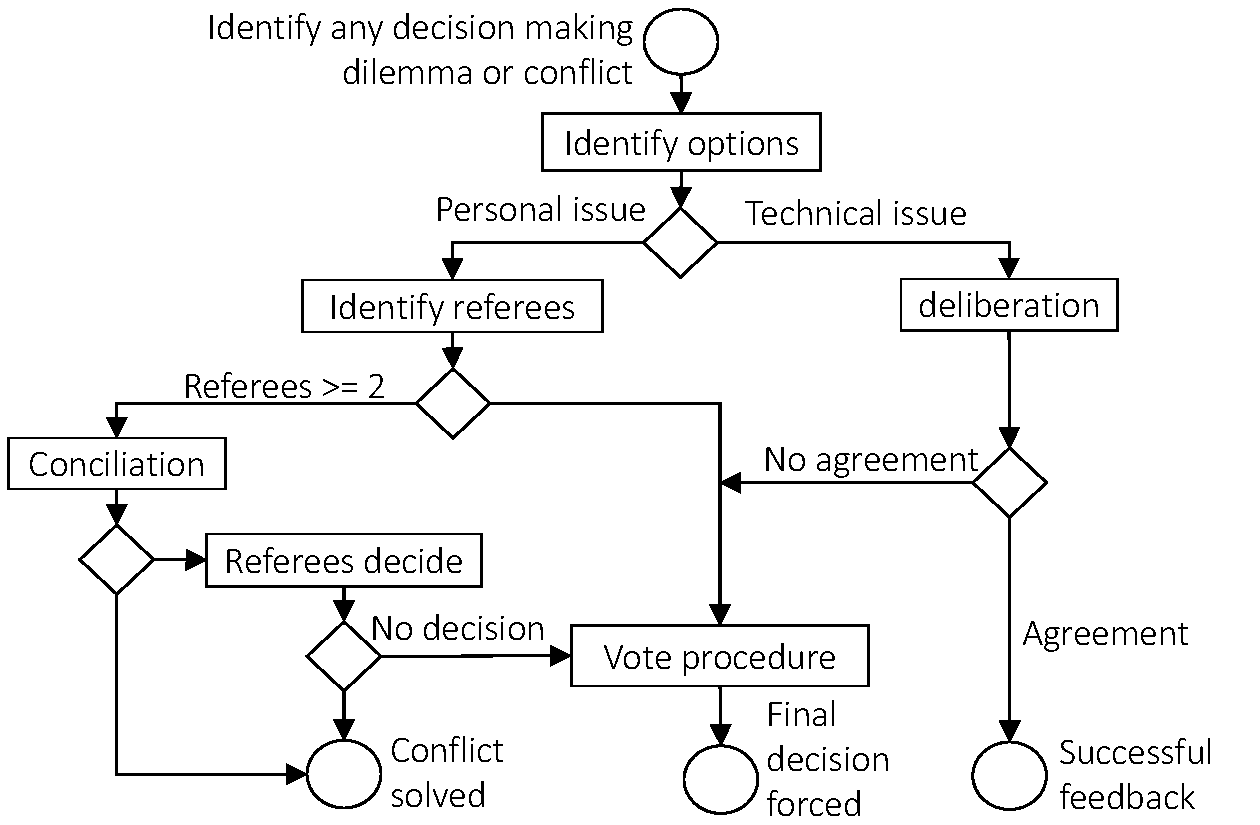
\includegraphics[width=0.6\textwidth]{figs/met}
	\caption{Decision Making and Conflicts Resolution Methodology}
	\label{fig:decisions}
\end{figure}



%DEA~\cite{charnes1978measuring} is a non-parametric method that determines efficiency estimates for a set of similar entities, called decision making units (DMU). 
%We refer to the set of DMUs as ${\cal K}:=\{\DMU_1, \DMU_2,\dots,\DMU_K\}$, where ${
%K = |\cK|}$. 





\bibliography{references}
\bibliographystyle{plain}
\end{document}
